% !TEX encoding = UTF-8 Unicode
\documentclass[a4paper, 12pt]{article}
\usepackage{graphicx}
\usepackage{amsmath}
\usepackage[brazil]{babel}
\usepackage[utf8]{inputenc}

\author{Seu nome}
\title{}

\linespread{1.5}


\begin{document}
%Capa
\begin{center}
\textbf{MINISTÉRIO DA DEFESA}\\
\textbf{EXÉRCITO BRASILEIRO}\\
\textbf{DEPARTAMENTO DE CIÊNCIA E TECNOLOGIA}\\
\textbf{INSTITUTO MILITAR DE ENGENHARIA}\\
\textbf{Programa de Engenharia de Defesa / PGED}

\vspace{2.5cm}

\begin{large}
\textbf{Proposta de Tema de Dissertação de Mestrado
\\Curso: Mestrado em Engenharia de Defesa}

\vspace{1.5cm}

\textbf{Titulo de seu trabalho}

\vspace{1.5cm}


\textbf{Orientador: Paulo Rosa, Ph.D}

\end{large}

\vspace{1.5cm}

\textbf{Aluno: Bruno da Silva Giovanini (ED 14106)}


\vspace{2cm}

\begin{small}
Data de Apresentação no PGED:\\
Rio de Janeiro, XX de mestal do ano tal
\end{small}

\end{center}


%Título
\newpage
\begin{large}
\section{Título da Dissertação}
\textbf{Título da Tese:}\\
\textbf{Titulo de sua tese}\\

\noindent\textbf{Título da Capa:}\\
\textbf{Titulo da capa}\\

\noindent\textbf{Área de Concentração:}\\
Tecnologias e Sistemas de Computação\\

\noindent\textbf{Linha de Pesquisa:}\\
Tecnologias para Tratamento e Transmissão da Informação\\
\end{large}

%Desenvolvimento do Texto
\newpage

\section{Introdução}

\subsection{Motivação}

A utilização de robôs voadores tanto em aplicações militares quanto civis vem aumentando e os desafios envolvidos em seu desenvolvimento estão atraindo as comunidades científica e industrial. Graças a isso, os veículos aéreos não tripulados (VANTs) têm se tornado cada vez mais populares. Tarefas como monitoramento de áreas alagadas, resgates em regiões de difícil acesso e inspeção de equipamentos perigosos, são aplicações que tornam os VANT's cada vez mais presentes no nosso cotidiano. 

Recentes avanços em processadores de baixo consumo de energia e na miniaturização dos componentes eletrônicos e sensores estão expandindo o campo de utilização para ambientes mais restritos. Veículos aéreos não tripulados de menor escala com decolagem e aterrissagem vertical, também chamados de Mini-VTOL (\textit{Mini vertical taking-off and landing}), apresentam muitas vantagens em ambientes desse tipo, devido sua flexibilidade e agilidade quando em movimento. Essas habilidades tornam possível sua utilização em tarefas como busca e resgate em prédios e inspeção de áreas fechadas sem colocar outras vidas em risco. Porém, áreas restritas aumentam o risco do choque entre o robô e os itens ali contidos, dado o espaço limitado para sobrevoo. Nesse contexto, um mecanismo de controle que evite colisões contra obstáculos se torna importante para aumentar a segurança do vôo e é o objeto dessa proposta. Acredita-se que, essa solução irá expandir o número dos possíveis campos de atuação de VTOL's para tarefas ainda consideradas perigosas, como sobrevoo em áreas com equipamentos críticos e sensíveis.



\subsection{Objetivo}

O propósito desse trabalho é controlar o desvio de obstáculos de um VTOL, um quadricóptero, de forma automática permitindo que sua operação mantenha o foco na missão global e evitar, assim, possíveis acidentes. Especificamente, propomos um método que consiste em estimar continuamente a trajetória futura do veículo, dada sua dinâmica, seu estado atual e o input de controle corrente. Além disso, através das medidas de sensores de distância embarcados, realizar uma comparação com a trajetória e identificar possíveis colisões. Se uma colisão é iminente, um novo controle é selecionado e o controle do operador é minimizado até que não exista possibilidade de colisão.


\subsection{Estrutura da Proposta}

A continuidade desta proposta está estruturada como segue. Inicialmente é discutida a revisão de literatura na seção \ref{sec:rev}. Após, os tópicos tutoriais relacionados estão descritos na seção \ref{sec:tutoriais}. Uma descrição do problema em questão é abordado na seção \ref{sec:prob} e metodologia proposta é descrita na seção \ref{sec:meto}. Em seguida, o cronograma de execução é mostrado na seção \ref{sec:crono}, a viabilidade da pesquisa na seção \ref{sec:viabilidade} e os resultados esperados na seção \ref{sec:resultados}. Por fim, na seção \ref{sec:conclusao}, é feita uma conclusão sobre o potencial dessa proposta. 

\newpage

\section{Revisão de Literatura}
\label{sec:rev}

Nos últimos anos, veículos aéreos não tripulados receberam uma maior atenção da comunidade científica. Muitos autores focaram na modelagem e no controle destes veículos \cite{Ye2006},  com especial destaque para os quadricópteros \cite{Altug2002}. Nesse contexto, estudos abrangentes sobre a configuração da plataforma, metodologias de modelagem, modelagem compreensiva não linear, os efeitos aerodinâmicos, identificação e simulação de um quadricóptero foram realizados \cite{Zhang2014} \cite{Gibiansky2010}. Por ser considerado um sistema complexo não linear, técnicas para controle de quadricópteros são também amplamente estudadas. \cite{Salih2010} desenvolveu um controle PID para um quadricóptero para obter estabilidade em vôo. Por outro lado, \cite{Nicol2008}, propôs uma rede neural adaptativa para estabilizar o quadricóptero levando em consideração erros de modelagem e distúrbios do vento.

A partir de um modelo conhecido, diversas são as aplicações em estudo. Para a maioria, como navegação autônoma, tarefas multiagentes e desvio de obstáculos, a estimação do estado do veículo é considerado um grande desafio \cite{Achtelik2009}. Quando se trata de ambientes \textit{indoors}, a visão computacional, que utiliza-se de câmeras e processamento de imagem para estimação, é uma das linhas de pesquisa sobre o problema \cite{Shen2013} \cite{Blosch2010} \cite{Shen2013a}. Outra linha utiliza-se de sensores estereoceptivos para tal tarefa, como ultra-som \cite{Roberts2007} e laser \cite{Grzonka2012}. Já para ambientes \textit{outdoors}, torna-se possível a utilização do Sistema de Posicionamento Global (GPS) e alguns trabalhos que utilizam essa tecnologia foram desenvolvidos, como  \cite{Hoffmann2004} e \cite{Wendel2006}.

%A plataforma Parrot Ar.Drone, 

Quando se fala especificamente sobre desvio de obstáculos em tempo real, esse campo é bastante explorado em robótica. Para resolver essa questão, várias são as abordagens que vem sido adotadas. Dentre elas, os métodos baseados em campos potenciais artificiais,  onde sensores de distância são usados e suas medidas tratadas como vetores de repulsão de forças \cite{Bouktir2008}, \cite{Nieuwenhuisen2013} e \cite{Borenstein1989}; o método de janelas dinâmicas, que incorpora a dinâmica do robô ao problema de forma elegante através da redução do espaço de busca das possíveis velocidades alcançáveis em um curto período de tempo (janela dinâmica) \cite{Fox1997} \cite{Saranrittichai2013}; método de obstáculos com velocidade, que define um conjunto de velocidades possíveis que resultaria em uma colisão entre o robô e um obstáculo se movendo em uma certa velocidade \cite{Fiorini1998} \cite{Claes2012} \cite{Berg2012}; método de estados de colisões inevitáveis, considerado um estado em que uma colisão eventualmente irá ocorrer, independente da trajetória a ser estabecida e que leva em conta a dinâmica tanto do robô quanto dos obstáculos, fixos ou móveis \cite{Fraichard2004}; dentre outros.   

Um trabalho semelhante ao aqui proposto foi realizado por \cite{Israelsen}, porém o ambiente e a posição dos obstáculos já eram previamente conhecidas e geometricamente pré-programadas, não sendo utilizado sensores de distância. \cite{Grzonka2012} também desenvolveu um quadricóptero totalmente autônomo em ambiente \textit{indoor}, utilizando para o desvio de obstáculos o sensor de varredura a laser em miniatura Hokuyo-URG, considerado o menor e mais leve sensor a laser disponível comercialmente. Já \cite{Becker2012} utilizou cinco sensores ultra-sônicos para tal. Porém, tanto \cite{Grzonka2012} quanto \cite{Becker2012} utilizaram plataformas desenvolvidas e testadas previamente em laboratório por alguns anos, tendo em mãos modelagens dos veículos já bem definidas.



\newpage

\section{Tópicos Tutoriais}
\label{sec:tutoriais}

Nessa seção serão abordados os principais aspectos teóricos envolvidos nessa proposta. Inicialmente, 
o quadricóptero, que é a plataforma de vôo a ser aqui estudada, será descrita juntamente com sua dinâmica de vôo. Após, os dispositivos embarcados e suas contribuições para o controle do vôo e, por fim, o controle PID e sua utilização para o controle de quadricópteros.

\subsection{O Quadricóptero}

\cite{Salih2010} define o quadricóptero como um veículo voador com quatro rotores com decolagem e aterrissagem vertical. Por sua vez, \cite{Gibiansky2010} define quadricóptero como uma classe de helicópteros com quatro rotores girando rapidamente para empurrar o ar para baixo e criar uma força para mantê-lo elevado e posicionados nas extremidades de um corpo quadrado. A Figura \ref{fig:quad} ilustra a plataforma Parrot ArDrone 2.0, um quadricóptero bastante estudado e utilizado no meio científico.

\begin{figure}[h]
	\centering
		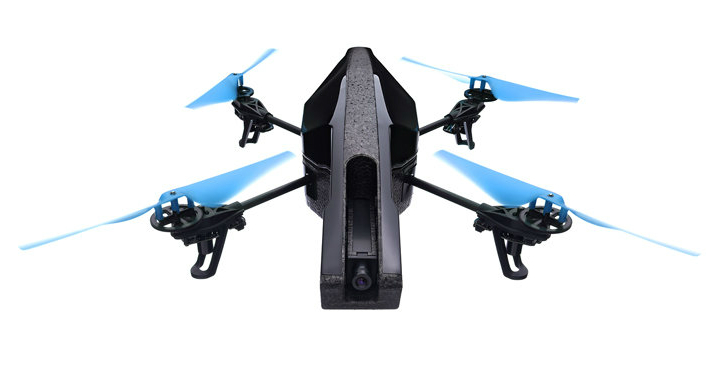
\includegraphics[scale=0.4]{img/parrot_drone.jpg}
	\caption{Plataforma Parrot Ardrone 2.0}
	\label{fig:quad}
\end{figure}

\noindent\textbf{Dinâmica de vôo}

O objetivo da dinâmica de vôo é manter a estabilidade do eixo central do quadricóptero,  controlando os quatro rotores que trabalham de forma independente. Esse processo é considerado complexo e precisa de apoio eletrônico para a execução \cite{Gibiansky2010}. A controladora de vôo é responsável por controlar a intensidade das rotações individualmente, de acordo com o movimento preterido. Um dos possíveis controles realizados pela controladora de vôo é o PID que será abordado em outra seção.

O quadricóptero é um sistema não linear, fortemente acoplado com seis graus de liberdade, onde três são movimentos lineares (x,y,z) e os outros três angulares ($\phi$,$\theta$,$\psi$). Porém, possui apenas quatro atuadores, sendo considerado então um sistema \textit{underactuated}, com dois movimentos lineares (x,y) dependentes dos movimentos angulares ($\phi$,$\theta$). As forças e momentos atuando no quadricóptero são produzidos pelas hélices ligadas aos rotores. Dois rotores rodam no sentido horário e dois no sentido anti-horário dispostos de forma à balancear o torque total do sistema \cite{Mian2008}. A Figura \ref{fig:diag quad} mostra o diagrama do corpo e os eixos de um quadricóptero.

Na Figura \ref{fig:diag quad}, \textit{l} representa a distância entre cada rotor e o centro, $\phi$, $\theta$ e $\psi$ representam os ângulos de Euler em relação aos eixos x, y e z, chamados de rolagem, afagem e guinada, respectivamente. Ti (i = 1, 2, 3, 4) é a força de empulso produzida por cada hélice e cada seta circular ao redor de Ti indica o sentido de rotação daquele rotor. O referencial inercial é denotado por E(X,Y,Z) e o referencial do corpo do quadricóptero é denotado por B(x,y,z). 

\begin{figure}[h]
	\centering
		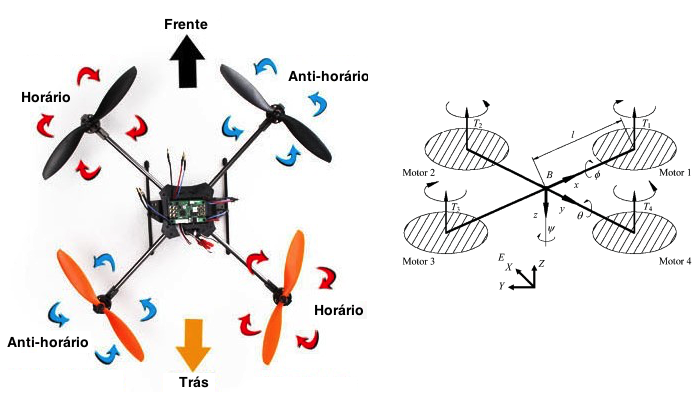
\includegraphics[scale=0.8]{img/diagrama_quadricoptero.png}
	\caption{Forças e momentos atuando em um quadricóptero.}
	\label{fig:diag quad}
\end{figure}

O aumento ou a diminuição da velocidade dos quatro rotores na mesma proporção irá gerar um movimento vertical. Quando os motores do par (1,3) operam independentemente e o par (2, 4) mantém a mesma velocidade, o ângulo de inclinação do par (1,3) em relação ao eixo y (afagem) poderá ser controlado e, indiretamente, poderá executar um movimento ao longo de seu eixo. Da mesma forma, a operação independente do par de motores (2,4), enquanto (1,3) com velocidade constante, poderá controlar o ângulo de rolagem em relação ao eixo x e um controle indireto do movimento ao longo do seu eixo também poderá ser feito. E, por fim, se ambos os pares possuírem velocidades independentes, o ângulo de guinada, em relação ao eixo z, poderá ser controlado. Dessa forma, o quadricóptero apresenta seis graus de liberdade. 

\subsection{Sistemas Embarcados de Navegação}

Navegação inercial é o processo pelo qual se adquirem informações sobre a posição, velocidade e atitude de um veículo com relação a um dado referencial, utilizando informações fornecidas por sensores inerciais tais como acelerômetros e giroscópios. Medindo-se as acelerações e velocidades angulares de um corpo, torna-se possível calcular as mudanças de velocidade, posição e atitude através de sucessivas integrações numericas \cite{Adalberto2009}.

A unidade de medida inercial, ou IMU, é o componente eletrônico onde são montados os sensores inerciais, sendo três acelerômetros, que fornecem as medidas das componentes da aceleração linear (x,y,z), e três giroscópios, sensores que fornecem as componentes da velocidade angular (por exemplo, arfagem, rolagem e guinada). Já a unidade de processamento é o componente responsável pelo processamento das medidas dos sensores inerciais. As velocidades lineares e as posições são obtidas a partir da integração dos sinais dos acelerômetros, enquanto que a integração dos sinais dos giroscópios fornece a atitude do veículo.  A Figura \ref{fig:imuStrap} ilustra a estrutura de um Sistema de Navegação Inercial acoplado a um veículo, composta por três giroscópios, três acelerômetros (x,y,z) e uma unidade de processamento (CPU) à esquerda e os movimentos gerados no quadricóptero à direita.

\begin{figure}[h]
	\centering
		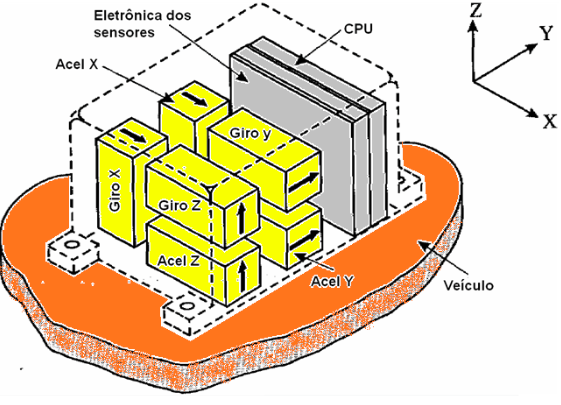
\includegraphics[scale=0.6]{img/imuStrap.png}
	\caption{Estrutura do Sistema de Navegação acoplada ao veículo (esquerda) e os movimentos gerados no quadricóptero (direita) }
	\label{fig:imuStrap}
\end{figure}

Magnetômetros podem ser incluídos em IMUs, permitindo uma melhor performance de cálculos de orientação em sistemas AHRS (do inglês, \textit{Attitude Heading Reference System}). Um sistema AHRS é composto de sensores que fornecem a orientação e atitude de uma aeronave. A principal diferença entre uma IMU e um AHRS é a adição de um sistema de processamento embarcado em um AHRS que fornece soluções de atitude e orientação, contra a IMU que apenas fornece os dados do sensor \cite{Angonese2013}.

A Figura \ref{fig:imuVANTIME} demonstra o protótipo de uma IMU desenvolvida para o projeto VANT-IME. No hardware desenvolvido foram utilizados, um acelerômetro que mede a aceleração do veículo e um giroscópio de três eixos para complementar o acelerômetro, obtendo-se assim, informações de velocidade angular em altas frequências, o que se faz necessário para estabilização de aeronaves movendo-se em alta velocidade. Entretanto, devido a erros de deriva dos giroscópios, erros de integração e ao ruído, a utilização de um magnetômetro se faz necessária, pois permite a medição do campo magnético no qual está inserido. As informações de todos os sensores são lidas, filtradas e então processadas para a estimação da atitude da aeronave \cite{Paixao2011}. As Figuras \ref{fig:imuVANTIME}a,  \ref{fig:imuVANTIME}b,  \ref{fig:imuVANTIME}c ilustram as leituras dos sensores inerciais e a figura 3.2d demostra o gráfico resultante após a filtragem e processamento das leituras dos sensores individuais.

\begin{figure}[h]
	\centering
		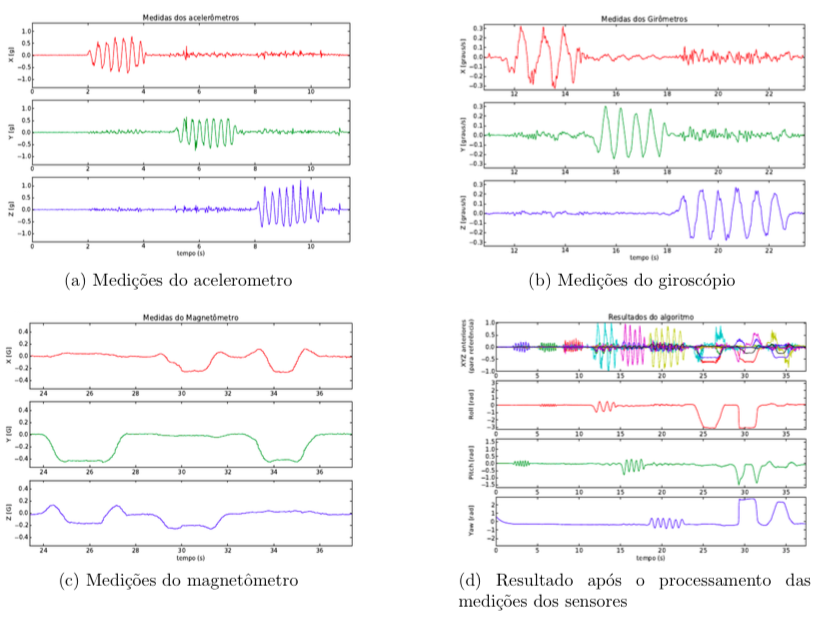
\includegraphics[scale=0.5]{img/imu_VANTIME.png}
	\caption{Gráfico das medições dos sensores inerciais da IMU do VANT-IME. Fonte \cite{Paixao2011}}
	\label{fig:imuVANTIME}
\end{figure}

\noindent\textbf{Acelerômetros e Giroscópios}

Acelerômetros são sensores que fornecem a medida e a força específica que atua no veículo, que é a resultante das ações da aceleração inercial e da aceleração da gravidade. Portanto, a partir da medida da força específica e do modelo do campo gravitacional da Terra, determina-se a aceleração linear, informação que é integrada para a determinação da velocidade e posição do veículo.

Giroscópios fornecem a medida da velocidade angular. Este dado é utilizado para a determinação da atitude do veículo. Já está na terceira geração. Esta, devido suas características de menor custo e volume, possibilitou sua utilização em grande escala em veículos de pequeno porte. Porém, sua exatidão é menor quando comparado às gerações anteriores. É formado por sensores baseados na tecnologia MEMS (\textit{Micro Electro Mechanical Systems}) que consistem em placas de cerâmicas vibrantes que utilizam Força de Coriolis para medir a taxa independente da aceleração \cite{Adalberto2009}. A Figura \ref{fig:imumems} mostra uma IMU tipo MEMS com acelerômetros e giroscópios embutidos. 

\begin{figure}[h]
	\centering
		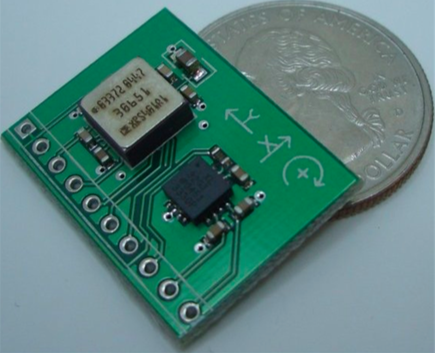
\includegraphics[scale=0.3]{img/imumems.png}
	\caption{IMU tipo MEMS da \textit{Spark Fun Electronics} SEN-00842}
	\label{fig:imumems}
\end{figure}

\subsection{Controle PID e quadricópteros}

\noindent\textbf{Controle PID}

Um controle PID é um método comum para controlar robôs e a sua utilidade está na aplicabilidade geral na maioria dos sistemas de controle, principalmente quando o modelo matemático de planta é complexo e não conhecido \cite{Ogata2003}. É um sistema de controle fechado que reage a mudanças no ambiente, que são captadas por sensores, e se baseia na constante sintonia das entradas para obter a saída esperada \cite{Kingdom}.  

O algoritmo de cálculo do controle PID envolve três parâmetros constantes: o valor proporcional (P), o valor integral (I) e o valor derivativo (D).

\begin{itemize}
\item
Valor proporcional - É tipicamente o erro. Ele é usualmente a distância que o robô deve viajar, ou a temperatura que se queira alcançar. Se o robô está na posição A, mas quer estar na posição B, então o valor proporcional P é $A - B$.
\item
Valor integral - É o acúmulo dos erros passados no tempo (t). Por exemplo, se o robô está continuamente fora da média por uma certa quantidade de tempo, o valor I irá tratar isso. Supondo que em $t_1$ o erro era A, em $t_2$ o erro era B e em $t_3$ o erro era C. o valor integral I seria $A/t_1 + B/t_2 + C/t_3$.
\item
Valor derivativo - É a mudança do erro no tempo (t). Por exemplo, se o erro era C e, depois do tempo t, passou a ser D, o valor derivativo D é $(C-D)/t$. Normalmente, o contador de tempo da microcontroladora é utilizado para medir esse tempo. Além disso, D é utilizado para predizer mudanças futuras baseando-se na taxa mudança atual.
\end{itemize}

A soma ponderada desses três termos é usada para ajustar o processo através de um elemento de controle, como uma válvula ou como o controle da quantidade de energia aplicada no sistema. O peso é atribuído através de uma constante K denominada ganho e tem o papel de ajustar os valores P, I e D. Ou seja, cada termo P, I e D possui o seu ganho associado e a equação básica de controle é dada pela equação \ref{eq:equacaoPID}

\begin{equation}
	\centering
		P*K_p + I*K_i + D*K_d	
	\label{eq:equacaoPID}
\end{equation}

A atuação do ganho no desempenho do sistema de controle PID pode ser visualizado na Figura \ref{fig:ganhoPID}, onde a linha azul indica o sinal de referência e as demais linhas indicam diferentes comportamentos com a variação dos ganhos $K_p$, $K_i$ e $K_d$. Um menor tempo de estabilização é normalmente desejável \cite{Kingdom}.  

\begin{figure}[h]
	\centering
		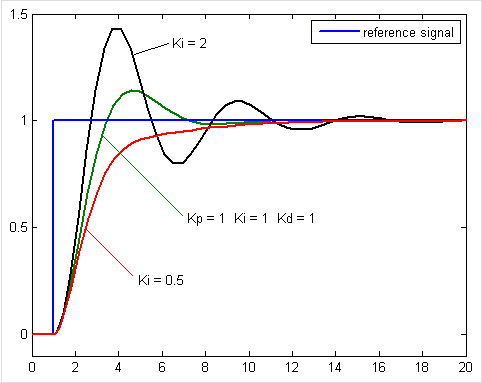
\includegraphics[scale=0.5]{img/ganho_PID.png}
	\caption{Desempenho do sistema para diferentes ganhos $K_p$, $K_i$ e $K_d$.}
	\label{fig:ganhoPID}
\end{figure}
 
\noindent\textbf{PID em quadricópteros}

A maioria dos quadricópteros utilizam PID para estabilização e permitem que o usuário altere os parâmetros para ajustar a performance \cite{Liang}. A Figura \ref{fig:PIDquad} ilustra o esquema de controle PID de um quadricóptero para a estabilização. Basicamente, o feedback é obtido através dos sensores do quadricóptero que são avaliados em conjunto com o movimento pretendido pelo piloto através do controle PID e, após, passado ao atuador como comando para os motores. 

\begin{figure}[h]
	\centering
		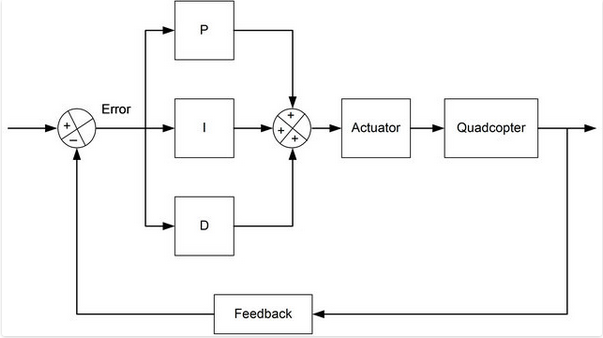
\includegraphics[scale=0.5]{img/PID_quad_geral.png}
	\caption{Controle PID de um quadricóptero.}
	\label{fig:PIDquad}
\end{figure}


Geralmente, segundo \cite{Liang}, existem ao todo três controles PID's, um para cada eixo ($\phi$,$\theta$,$\psi$) e a alteração dos valores dos ganhos ($K_p$, $K_i$ e $K_d$) de cada eixo acarretará em mudanças na reação do quadricóptero quando sujeito a interferências externas. A Figura \ref{fig:PIDaxis} ilustra a estrutura do controle PID de um eixo.

%\begin{itemize}
%\item
%$K_p$ - O quadricóptero pode voar de forma estável somente com esse ganho. Ele determina qual é mais importante, o controle humano ou os valores medidos pelo giroscópio. Quanto maior o coeficiente, mais sensível e reativo ele será para mudanças de ângulos. Se muito pequeno, mais lento e difícil de mantê-lo estável.
%\item
%$K_i$ - Pode aumentar a precisão da posição angular. O tempo de reação à uma alteração do ângulo de inclinação é afetada.
%\item
%$K_d$ - Permite ao quadricóptero alcançar a atitude desejada mais rapidamente. Ele amplifica a ação do usuário. 

%\end{itemize}

\begin{figure}[h]
	\centering
		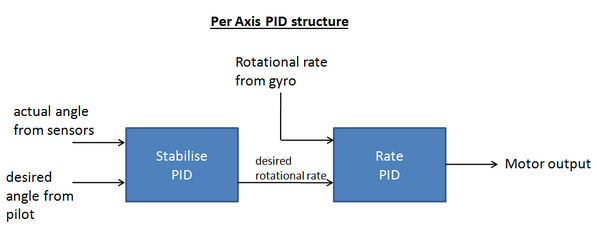
\includegraphics[scale=0.6]{img/PID_quad_axis.png}
	\caption{Controle PID por eixo.}
	\label{fig:PIDaxis}
\end{figure}



\newpage

\section{O Problema:}
\label{sec:prob}
\noindent\textbf{Segurança em voo para quadricoptero}

Em linhas gerais, o problema a ser tratado é evitar que o quadricóptero se choque durante sua navegação. A operação desta plataforma não é uma tarefa simples e exige muito treinamento e prática para uma operação segura sem colisões. Daí a importância de um sistema de desvio de obstáculos automático. 

\noindent\textbf{Formulação do Problema}

Considerando um quadricóptero como um robô com uma dinâmica não linear genérica em um espaço arbitrário, $\mathcal{X} \subset R^{n}$ o seu espaço de estados e $\mathcal{U} \subset R^{n}$ o espaço do input de controle. Em tempo contínuo, a dinâmica do robô é uma função em $\mathbf{f} \in \mathcal{X} \times \mathcal{U} \times R \rightarrow R^{n}$ e é dada pela relação \ref{eq:equacaoDinProb}:

\begin{equation}
\centering
\dot{\mathbf{x}} = \mathbf{f}(\mathbf{x}(t),\mathbf{u}(t),t)  
\label{eq:equacaoDinProb}
\end{equation}

\noindent onde $t$ é o tempo, $\mathbf{x}(t)$ é o estado do robô no tempo $t$ e $\mathbf{u}(t)$ é o input de operação no tempo $t$. Consequentemente, dado um estado inicial $\mathbf{x_0} = \mathbf{x}(0)$ e uma constante de input de operação $\mathbf{u}$, o estado do robô em um instante $t > 0$ é dado pela relação \ref{eq:equacaoPosProb}:
 

\begin{equation}
\centering
\mathbf{x} = \mathbf{g}(\mathbf{x},\mathbf{u},t)  
\label{eq:equacaoPosProb}
\end{equation}

\noindent onde $\mathbf{g} \in \mathcal{X} \times \mathcal{U} \times R \rightarrow \mathcal{X}$ representa a solução da equação diferencial \ref{eq:equacaoDinProb}.

Porém, quando se considera um ambiente repleto de obstáculos, o espaço de estados do robô se restringe à posições não ocupadas por eles. Define-se então $\mathcal{O} \subset R^3$, como a subárea do espaço $R^n$ de movimentos possíveis do robô ocupada por obstáculos e as regiões que estão escondidas por eles quando vistas pelo estado corrente do robô. Além disso, $\mathcal{R}(x)$, como a subárea ocupada pelo robô no estado $x \in \mathcal{X}$. Assim, o problema passa a ser definido como identificar a menor variação necessária  $\Delta\mathbf{u} \in \mathcal{U}$ sobre o controle de operação $\mathbf{u}$, dado o atual estado $\mathbf{x}$ do robô, a fim de que se evite uma colisão com algum obstáculo em qualquer momento até se alcançar um período previamente definido $\tau \in R$ conforme a relação \ref{eq:equacaoProb}:

\begin{equation}
\begin{aligned}
\text{min: }& \Delta\mathbf{u} \\
\text{Sujeito a: }& \forall t \in [0,\tau], \mathcal{R}(\mathbf{g}(\mathbf{x}, \mathbf{u}+\Delta\mathbf{u}, t)) \cap \mathcal{O} = \emptyset
\end{aligned}
\label{eq:equacaoProb}
\end{equation}

%\Delta\mathbf{u^T}T\mathbf{u}

%\noindent onde $T \in R^{m \times m}$ é uma matriz positiva de pesos.

\newpage

\section{Metodologia}
\label{sec:meto}

A Figura \ref{fig:etapasMetodo} ilustra as etapas envolvidas no método desta proposta. As caixas em azul indicam os responsáveis pela aquisição dos dados necessários Sensores ultra-sônicos, os comandos de controle e a os sensores da IMU. Em verde, estão os processos de tratamento dos dados a fim de se obter medidas confiáveis para os módulos. Já em amarelo estão os módulos centrais de detecção de obstáculos e para evitar colisões. Eles estão separados para serem independentes e passíveis de substituição sem interferência no funcionamento do outro. Por fim, em vermelho está o controle de atitude, que é um dos processos do controle de vôo, e que receberá comandos e os transformarão em algum comportamento do quadricóptero.   

\begin{figure}[h]
	\centering
	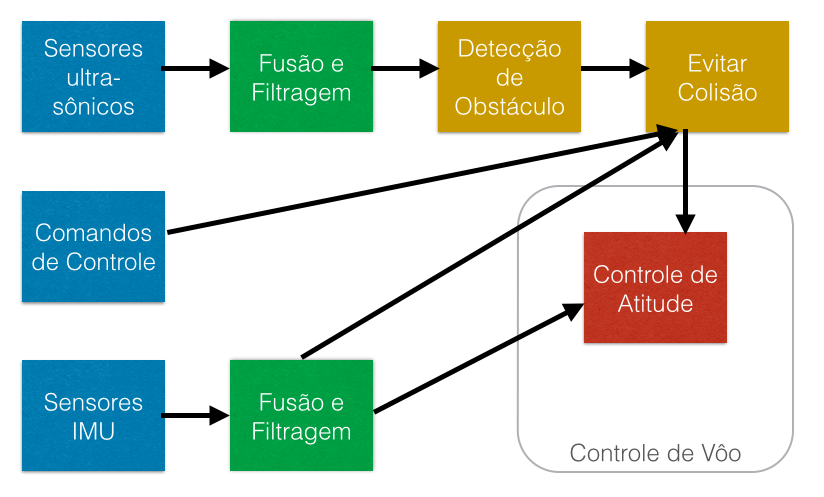
\includegraphics[scale=0.4]{img/etapasMetodo.png}
	\caption{Etapas do método}
	\label{fig:etapasMetodo}
\end{figure}

\newpage

\section{Cronograma} 
\label{sec:crono}
Para facilitar a compreensão do projeto, optou-se por dividir o projeto em módulos que seguirão o cronograma abaixo.
\begin{figure}[h]
	\centering
		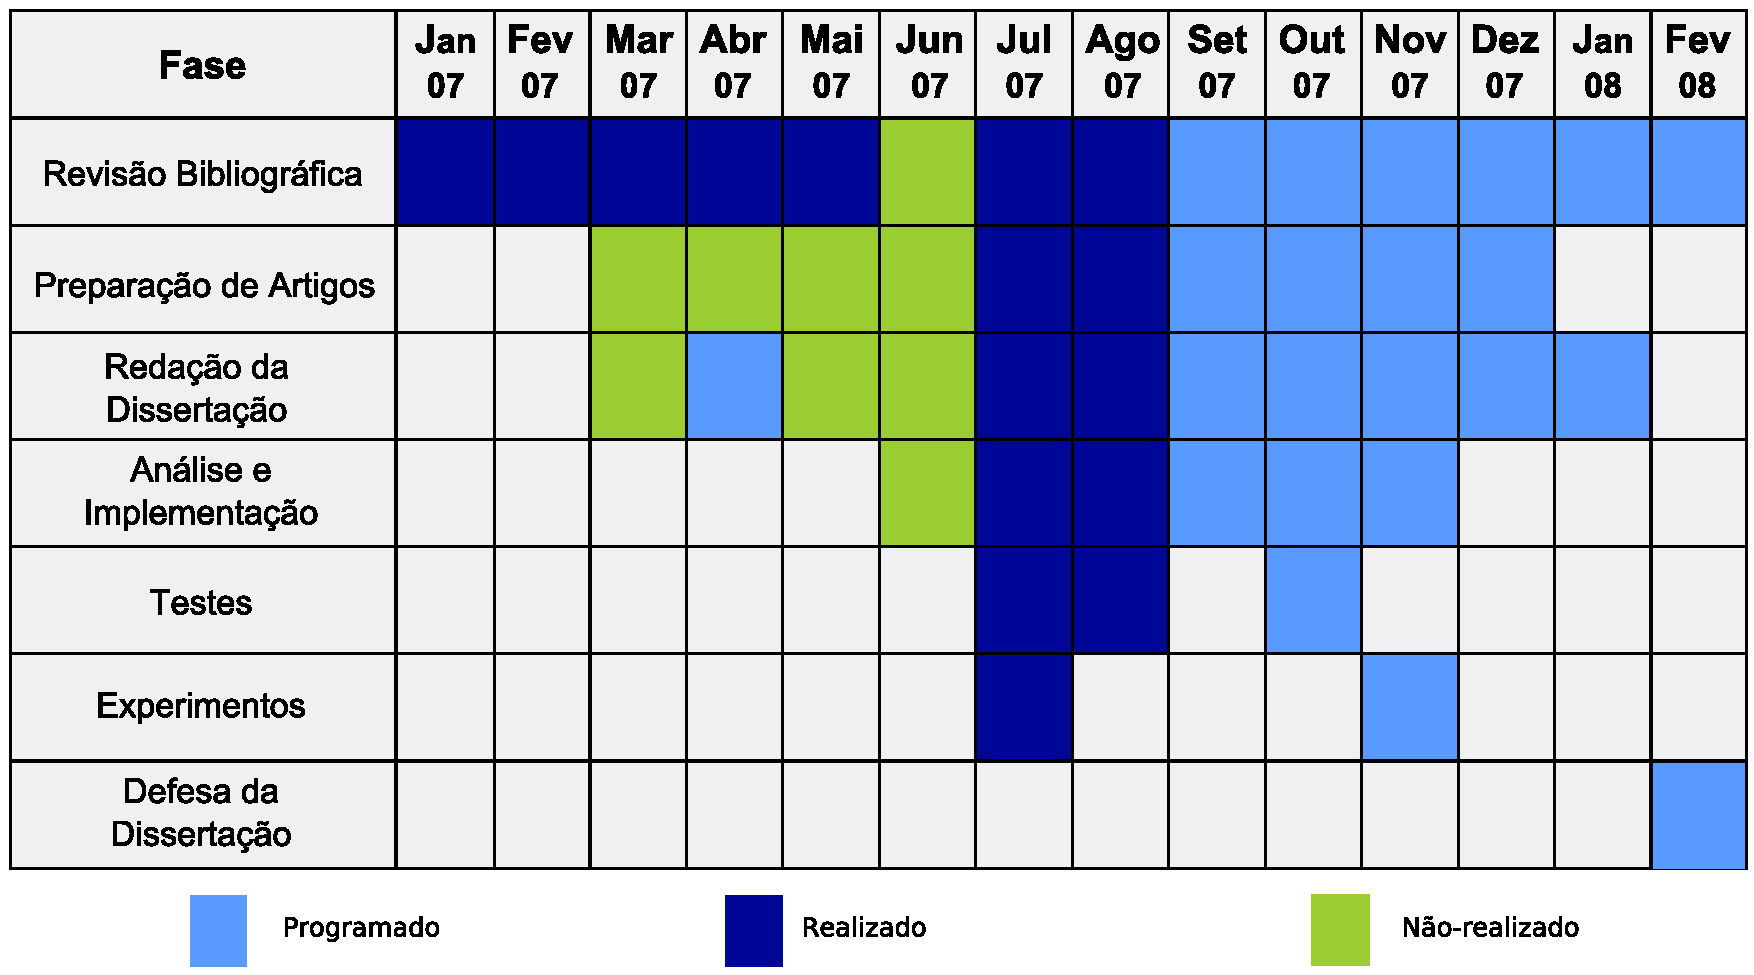
\includegraphics[scale=0.4]{img/cronograma.pdf}
	\caption{Cronograma físico.}
	\label{fig:cronograma}
\end{figure}

\newpage

\section{Viabilidade da Pesquisa}
\label{sec:viabilidade}

\newpage

\section{Resultados Esperados}
\label{sec:resultados}

\newpage

\section{Conclusão}
\label{sec:conclusao}

\newpage

\bibliographystyle{abbrv}
\bibliography{Dissertacao} 

\newpage

\begin{center}
\_\_\_\_\_\_\_\_\_\_\_\_\_\_\_\_\_\_\_\_\_\_\_\_\_\_\_\_\_\_\_\_\_\_\_\_\_\_\_\_\_\_\_\_\_\_\_\_\_\_\_ \\

Bruno da Silva Giovanini (ED 14106) \\Aluno \\ 
 
\hspace{4cm}
\\


\_\_\_\_\_\_\_\_\_\_\_\_\_\_\_\_\_\_\_\_\_\_\_\_\_\_\_\_\_\_\_\_\_\_\_\_\_\_\_\_\_\_\_\_\_\_\_\_\_\_\_ \\
Paulo Rosa, Ph.D \\Orientador \\ 

\hspace{4cm}
\\


\_\_\_\_\_\_\_\_\_\_\_\_\_\_\_\_\_\_\_\_\_\_\_\_\_\_\_\_\_\_\_\_\_\_\_\_\_\_\_\_\_\_\_\_\_\_\_\_\_\_\_ \\
Maj Ronaldo Moreira Salles, Ph.D \\Coordenador de Pós-Graduação \\

\hspace{4cm}

\end{center}
Concordo com a presente Proposta de Dissertação e declaro que as necessidades para sua execução serão garantidas pelo departamento. \\
IME, em \today
 \hspace{4cm}
 \\
 \\
 \\
 \\
 
\begin{center}
\_\_\_\_\_\_\_\_\_\_\_\_\_\_\_\_\_\_\_\_\_\_\_\_\_\_\_\_\_\_\_\_\_\_\_\_\_\_\_\_\_\_\_\_\_\_\_\_\_\_\_\_\_\_\_\_\_\_\_ \\
Antonio Carlos Freire de Almeida, Ten Cel QEM, \\
CHEFE SE/8
\end{center}


\end{document}